\documentclass[xcolor=x11names,compress]{beamer}
\usepackage[english]{babel}

%% General document %%%%%%%%%%%%%%%%%%%%%%%%%%%%%%%%%%
\usepackage{graphicx}
\usepackage{tikz}
\usepackage{wrapfig}
\usepackage{hyperref}
\usepackage{fancybox}
\usepackage{amsthm}

\usetikzlibrary{arrows}
\tikzstyle{block}=[draw opacity=0.7,line width=1.4cm]
\usetikzlibrary{decorations.fractals}
%%%%%%%%%%%%%%%%%%%%%%%%%%%%%%%%%%%%%%%%%%%%%%%%%%%%%%


%% Beamer Layout %%%%%%%%%%%%%%%%%%%%%%%%%%%%%%%%%%
\useoutertheme[subsection=false,shadow]{miniframes}
\useinnertheme{default}
\usefonttheme{serif}
\usepackage{palatino}

\setbeamerfont{title like}{shape=\scshape}
\setbeamerfont{frametitle}{shape=\scshape}

\setbeamercolor*{lower separation line head}{bg=DeepSkyBlue4} 
\setbeamercolor*{normal text}{fg=black,bg=white} 
\setbeamercolor*{alerted text}{fg=red} 
\setbeamercolor*{example text}{fg=black} 
%Responsible for colour of slide titles, bullets etc.  
\setbeamercolor*{structure}{fg=DeepSkyBlue4!50!black} 
% 
\setbeamercolor*{palette tertiary}{fg=black,bg=black!10} 
\setbeamercolor*{palette quaternary}{fg=black,bg=black!10} 


\newenvironment<>{problock}[1]{%
  \begin{actionenv}#2%
      \def\insertblocktitle{#1}%
      \par%
      \mode<presentation>{%
        \setbeamercolor{block title}{fg=white,bg=DeepSkyBlue4}
       \setbeamercolor{block body}{fg=black,bg=black!10}
       \setbeamercolor{itemize item}{fg=blue!20!black}
       \setbeamertemplate{itemize item}[triangle]
     }%
      \usebeamertemplate{block begin}}
    {\par\usebeamertemplate{block end}\end{actionenv}}


\useinnertheme[shadow=true]{rounded}


\renewcommand{\(}{\begin{columns}}
\renewcommand{\)}{\end{columns}}
\newcommand{\<}[1]{\begin{column}{#1}}
\renewcommand{\>}{\end{column}}
%%%%%%%%%%%%%%%%%%%%%%%%%%%%%%%%%%%%%%%%%%%%%%%%%%
\newcommand{\hlb}[1]{\textbf{\textcolor{blue}{#1}}}
\newcommand{\hl}[1]{\textcolor{blue}{#1}}
\newcommand{\lien}[2]{\mathcal{L}_{#1}^{#2}}
\newcommand{\lie}[1]{\mathcal{L}_{#1}}

\newcommand{\colv}[2]{\begin{pmatrix}#1\\#2\end{pmatrix}}

%\usepackage[english]{babel}
\usepackage[utf8]{inputenc}
%\usetheme{Goettingen}

\begin{document}
\title{Bifurcations in continuous time dynamical systems}
\author{Debsankha Manik}

\begin{frame}
\titlepage
\end{frame}

\section{Recap}

\begin{frame}{Hard impact in an oscillating system}

\begin{figure}
\caption{}
\begin{center}
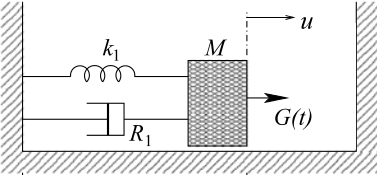
\includegraphics[width=0.4\columnwidth]{../2013-02-15/hardcol}
\end{center}
\end{figure}

The equation of motion:
\begin{equation}
\label{eq:driven}
\ddot{x}+\gamma\dot{x}+\omega_0^2x=F\cos{\omega t}
\end{equation}

Switching manifold:
If $x=\sigma$,
\begin{eqnarray*}
x&\mapsto& x\\
v&\mapsto& -v
\end{eqnarray*}
\end{frame}

\begin{frame}
The solution to equation \eqref{eq:driven} is a sum of two parts: a 
\emph{particular solution} that is independent of the initial conditions, and 
a \emph{homogeneous solution} that is dependent on the initial conditions.  

To be more precise:
\begin{eqnarray*}
x_p(t)&=&\frac{F}{\sqrt{(\omega_0^2-\omega^2)^2+\omega^2\gamma^2}}cos(\omega t+tan^{-1}\frac{\omega \gamma}{\omega^2-\omega_0^2})\\
x_h(t)&=&\frac{e^{-\gamma t/2}}{\omega_g}\left\{(\omega_g\cos{\omega_gt}+\frac{\gamma}{2}\sin{\omega_gt})x_0 + (\sin{\omega_gt})v_0 \right\}\\
\omega_g&=&\sqrt{\omega_0^2-\frac{\gamma^2}{4}}
\end{eqnarray*}
\end{frame}


\begin{frame}{Dependence of transience on $F$}
\begin{figure}
\begin{center}
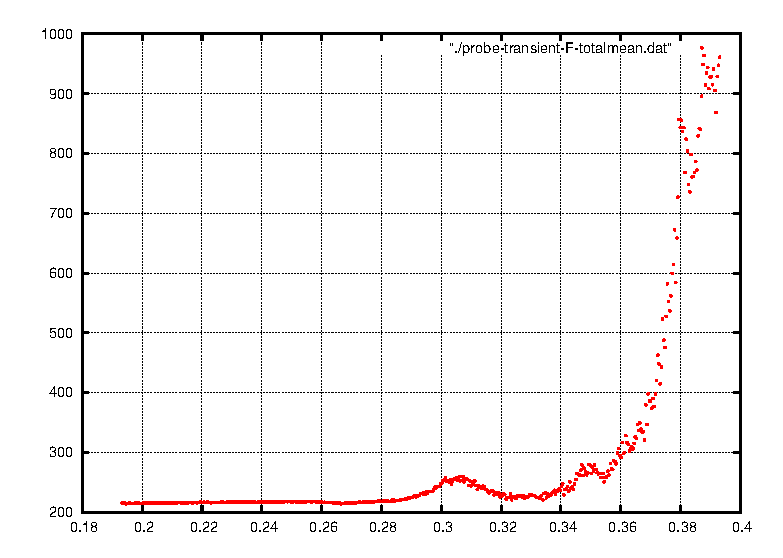
\includegraphics[width=0.9\columnwidth]{../2013-01-28/probeF}
\end{center}
\end{figure}
\end{frame}

\begin{frame}{Dependence of transience on $\gamma$}
\begin{figure}
\begin{center}
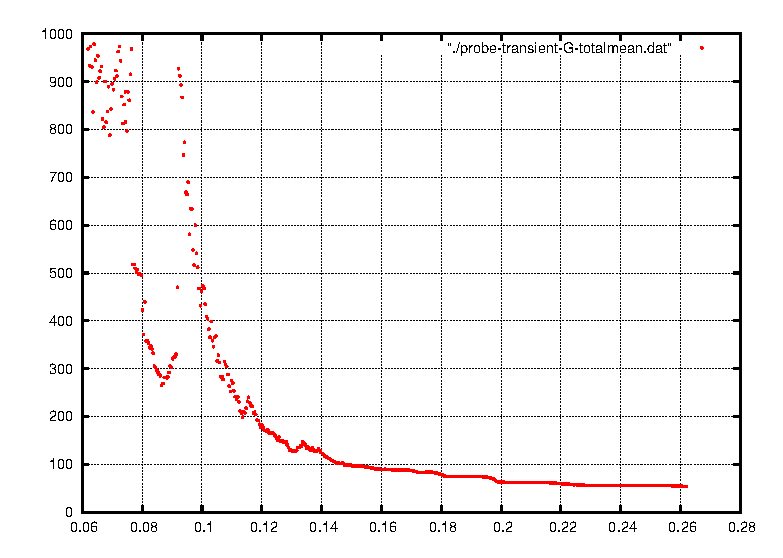
\includegraphics[width=0.9\columnwidth]{../2013-01-28/probeG}
\end{center}
\end{figure}
\end{frame}

\section{Types of trajectories}
\begin{frame}{The poincare map(a projection)}
\begin{figure}
\begin{center}
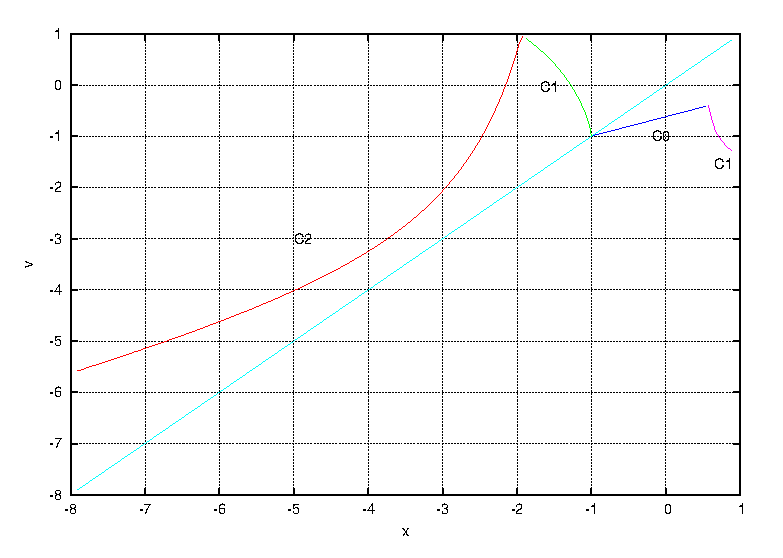
\includegraphics[width=0.9\columnwidth]{map1-coloured}
\end{center}
\end{figure}
\end{frame}

\begin{frame}{2 collisions}
\begin{figure}
\begin{center}
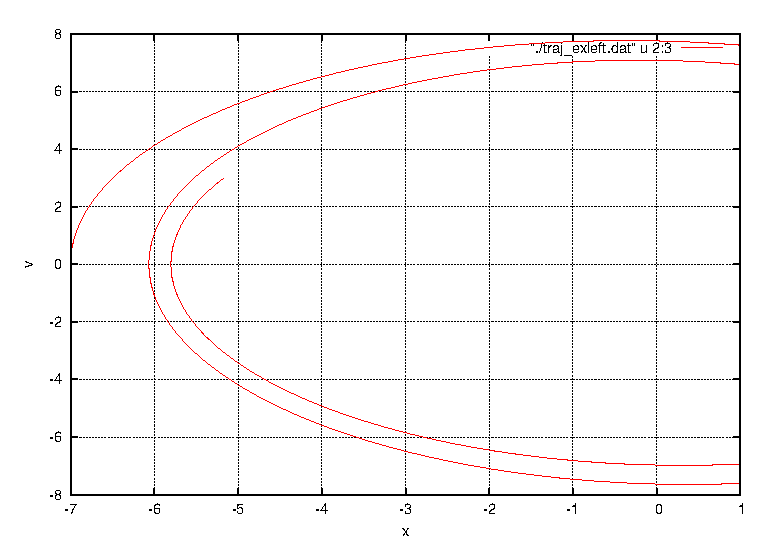
\includegraphics[width=0.9\columnwidth]{traj_exleft}
\end{center}
\end{figure}
\end{frame}

\begin{frame}{Grazing 1}
\begin{figure}
\begin{center}
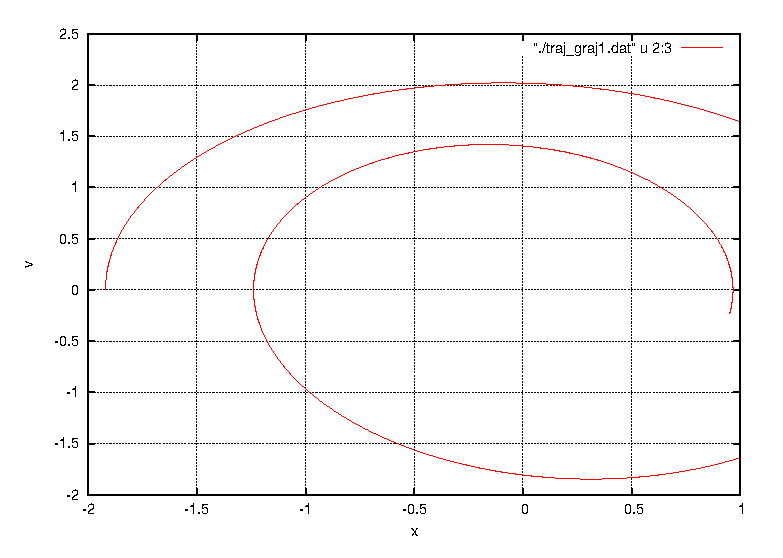
\includegraphics[width=0.9\columnwidth]{traj_graj1}
\end{center}
\end{figure}
\end{frame}

\begin{frame}{Grazing 2}
\begin{figure}
\begin{center}
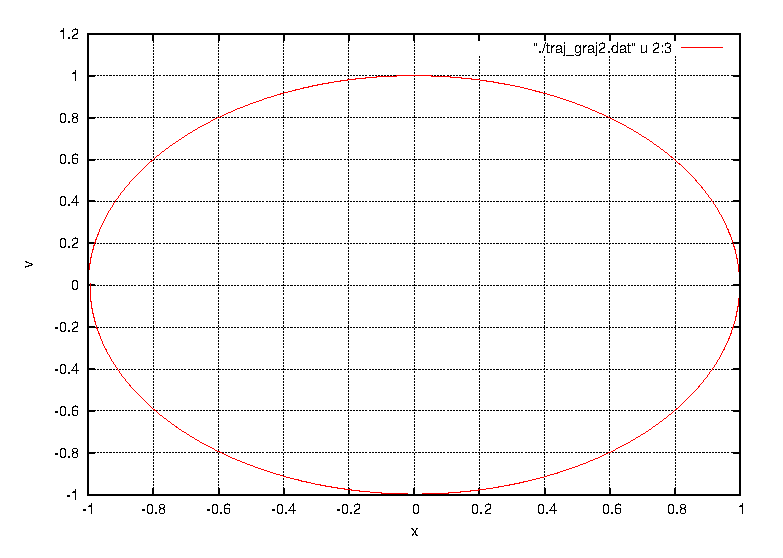
\includegraphics[width=0.9\columnwidth]{traj_graj2}
\end{center}
\end{figure}
\end{frame}

\begin{frame}{Grazing 3}
\begin{figure}
\begin{center}
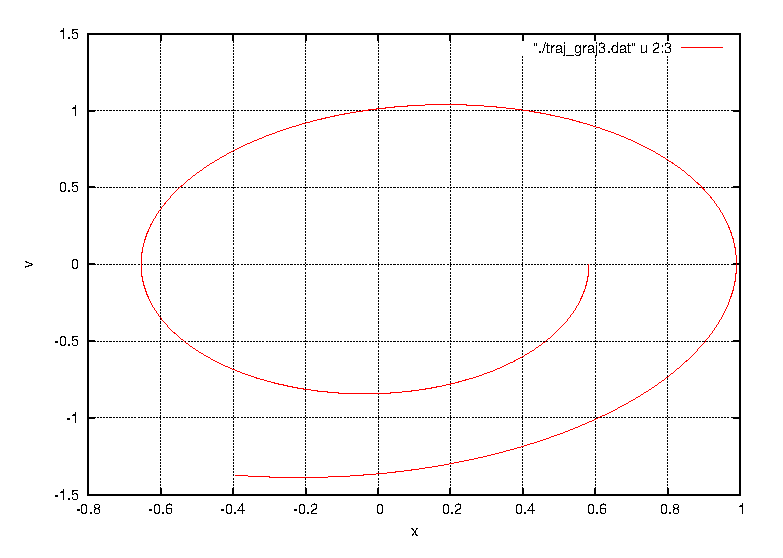
\includegraphics[width=0.9\columnwidth]{traj_graj3}
\end{center}
\end{figure}
\end{frame}

\begin{frame}{1 collision}
\begin{figure}
\begin{center}
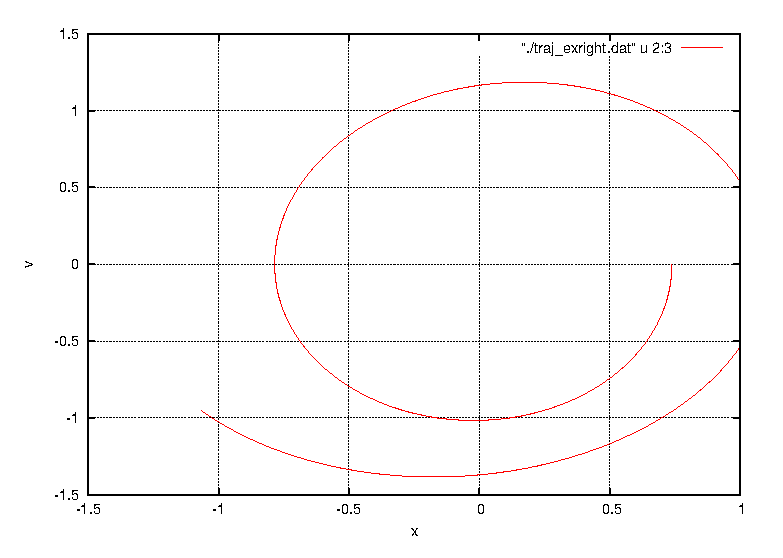
\includegraphics[width=0.9\columnwidth]{traj_exright}
\end{center}
\end{figure}
\end{frame}

\begin{frame}{Drawbacks of the projection}
\begin{figure}
\begin{center}
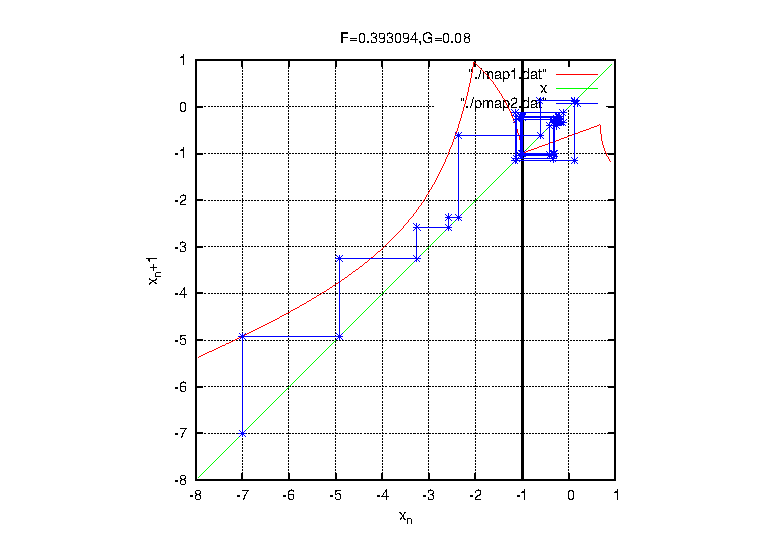
\includegraphics[width=0.9\columnwidth]{before-grazing-period-3}
\end{center}
\end{figure}
\end{frame}

\begin{frame}
\begin{itemize}
\item Even before the stable orbit grazes, we see higher periodic orbts.  
Previously we thought it is due to a temporary lock-in to a pseudo periodic 
orbit due to intremittency.   
\item We saw that the cause is not intermittency, but rather the periods 
getting locked on to what looks like a genuine periodic orbit.  We saw 
period 3.
\item At the same time, the period-1 fixed point exists and is stable, just 
the basin of attraction not filling up the whole phase space.
\item How does the basin boundary look? 
\item We tried  to plot it by taking many initial conditions and following the 
trajectories to 'paint' the phase space.  
\item It does not work.  Since the system is non-autonomous, later 
trajectories overwrite the colors painted by previous trajectories.  
\end{itemize}
\end{frame}

\begin{frame}<article>	%Cool way of hiding frames from presentation
\begin{itemize}
\item The map we plotted by starting from $\vec{x}(\varphi)=(x_0,0)$ and 
obtaining $\vec{x}(T+\varphi)$, does not seem to capture the full story.  
This is not surprising, because we are taking projections.  

\item However, 
what about the long transients before stabilizing onto the period-1 FP's then? 
Are they to be taken to be normal artefact of the wall? We could plot the 
transient times solely for period-1.  We did, for $\tau vs. F$, the bumps 
persist even there.  

\item The linear region in the $x_{n}$ vs.   $x_{n+1}$ plot keeps shrinking as 
we approach grazing.  Could that signify the increase in transient time? Keep 
in mind that the 2-D projection of the 4-D map onto the $v_n=0$ plane does not 
contain the full picture anyway.  \end{itemize}
\end{frame}

\section{Collision detector}
\begin{frame}{The collision detector}
The previous strategy of determining the basin boundary of period-1 orbit did 
not work due to the extra dimension: time.  \\
\vspace{1em}
But we know that Poincáre sections can be used to take care of extra dimensions.  \\

\vspace{1em}
Also, what if we don't look for ``basin boundary'' as such, but some area in 
the $v\times x$ space which merely \emph{guarantees} a period one orbit? In 
other words, a sufficient, but not necessary condition for period-1 orbit, 
which has the added advantage of being more tractable.  \\

\end{frame}

\begin{frame}{A sufficient condition}
Consider an initial condition:\footnote{Taking a slice through the time dimension}
\begin{align*}
\vec{x_p}(0)&=(-A,0)\\
\vec{x_h}(0)&=(x_0,v_0)
\end{align*}

Where $A=\frac{F}{\sqrt{(\omega_0^2-\omega^2)^2+\omega^2\gamma^2}}$

Starting from this point, the solution is, as usual:
\[
x(t)=-A\cos{\omega t}+\frac{e^{-\gamma t/2}}{\omega_g}\left\{(\omega_g\cos{\omega_gt}+\frac{\gamma}{2}\sin{\omega_gt})x_0 + (\sin{\omega_gt})v_0 \right\}
\]

\end{frame}

\begin{frame}{Akin to decaying beats}
\begin{figure}
\begin{center}
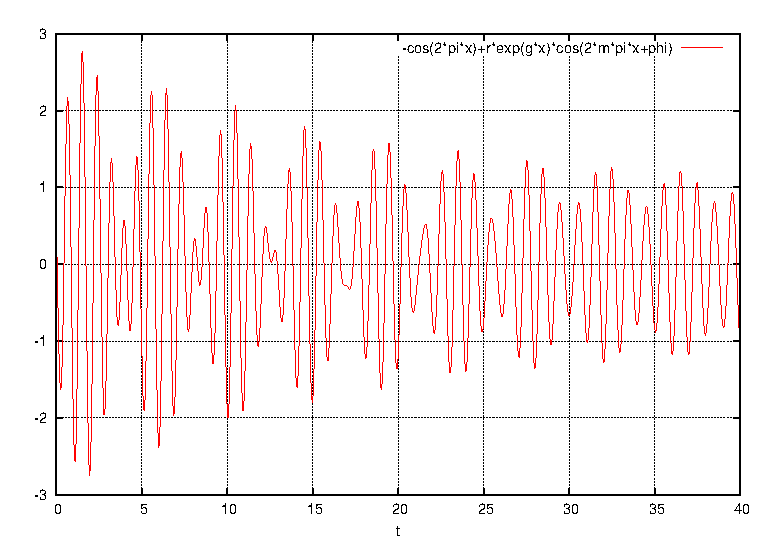
\includegraphics[width=0.8\columnwidth]{beats-decaying}
\end{center}
\end{figure}
\end{frame}

\begin{frame}{A little tidying up}

\begin{align*}
x(t)&=-A\cos{\omega t}+\frac{e^{-\gamma t/2}}{\omega_g}\left\{(\omega_g\cos{\omega_gt}+\frac{\gamma}{2}\sin{\omega_gt})x_0 + (\sin{\omega_gt})v_0 \right\}\\
&=-A\cos{\omega t}+e^{-\gamma t/2}B\cos{\left(\omega_g t+C\right)}\\
C&=-tan^{-1}\frac{\frac{\gamma}{2\omega_g}x_0+\frac{v_0}{\omega_g}}{x_0}\\
B&=\sqrt{x_0^2+\left(\frac{\gamma}{2\omega_g}x_0+\frac{v_0}{\omega_g}\right)^2}
\end{align*}
\end{frame}

\begin{frame}{Predicting collisions}
In general, the sum of two different sine waves differing both in amplitude 
and frequency cannot be further simplified.  However, an approximate envelope 
can be calculated.  
\begin{figure}
\begin{center}
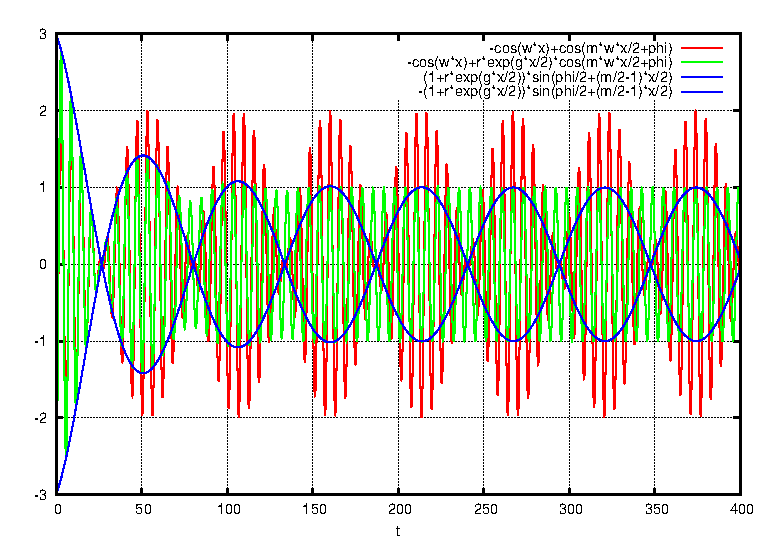
\includegraphics[width=0.8\columnwidth]{guess_envelope}
\end{center}
\end{figure}
\end{frame}

\begin{frame}

Now the job is simple:
\begin{enumerate}
\item Consider the $x_0\times v_0$ space.  
\item For any point in the space, using the envelope, predict if there will be 
any future collision or not.  
\item Points for which there is no further collision should form a closed area 
in the whole space.  
\item The area must shrink as we approach grazing.  
\item Correlate the area with transient lifetime. 
\end{enumerate}
\end{frame}


\begin{frame}[label=envelope-guess]
The trajectory:
\begin{equation}
x(t)=-A\cos{\omega t}+e^{-\gamma t/2}B\cos{\left(\omega_g t+C\right)}
\end{equation}
\hyperlink{envelope-proof}{\beamergotobutton{back}}
Will have an envelope:\footnote{There are some aberrations in the first bulge 
of the envelope}
\begin{equation}
\label{eq-envelope}
E(t)=\left\{A+Be^{-\gamma t/2}\right\}\sin{\left( \frac{C+(\omega_g-\omega)t}{2} \right)}
\end{equation}
If $\omega \approx \omega_g$
\hyperlink{envelope-am}{\beamergotobutton{Other cases}}


The next peak of the envelope occurs at
\begin{equation}
\label{eq-tcol}
t_c= \left\{
\begin{matrix}
\frac{\pi-C}{\omega_g-\omega}\hspace{1em} \text{if }\omega_g>\omega\\
\frac{\pi+C}{\omega-\omega_g}\hspace{1em} \text{if }\omega_g<\omega
\end{matrix}
\right.  
\end{equation}

And has height:
\begin{equation}
\label{eq-nextcolheight}
E_{m}=A+Be^{-\gamma t_c/2}
\end{equation}

\end{frame}

\begin{frame}{Some definitions}
\begin{definition}
$E_m= $ height of the next peak of the envelope.  
\end{definition}

\begin{definition}
$x_m= $ height of the next peak of the trajectory  \footnote{Except in 
some cases, $x_m=E_m$}
\end{definition}

\begin{definition}
$\mu_{xv}=\left\{(x,v)\in\mathbb{X\times V}:x_m(x,v)<\sigma\right\}$
\end{definition}
\end{frame}


\begin{frame}{Some Useful Inequalities}
\begin{align}
t_c&\leq \frac{3\pi/2}{|\omega_g-\omega|}\\
x_m&\geq E_m\\
E_m&\geq A+Be^{-\gamma \frac{3\pi/4}{|\omega_g-\omega|}}\\
B&\geq max\left\{|x_0|,\left|\frac{\gamma}{2\omega_g}x_0+\frac{v_0}{\omega_g} \right|  \right\}\\
\mu_{xv}&\leq\left\{ (x,v): B\leq (\sigma-A)e^{\gamma \frac{3\pi/4}{|\omega_g-\omega|}}=\chi\right\}\\
&\leq\left\{ (x,v): -\chi \leq x\leq \chi, -\chi\omega_g-\frac{\gamma x}{2} \leq v\leq \chi\omega_g-\frac{\gamma x}{2}    \right\}
\end{align}


\end{frame}


\section{No-collision area}

\begin{frame}[label=muvsf]{$\mu_{xv}$Vs.  $F$}
\begin{figure}
\begin{center}
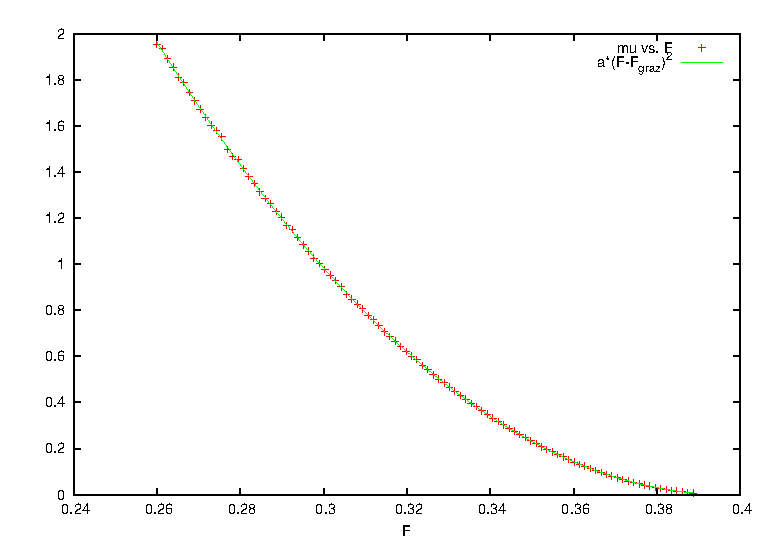
\includegraphics[width=0.8\columnwidth]{scanf}
\end{center}
\end{figure}
\hyperlink{avgtvsf}{\beamergotobutton{back}}
\end{frame}


\begin{frame}[label=muvsg]{$\mu_{xv}$Vs.  $\gamma$}
\begin{figure}
\begin{center}
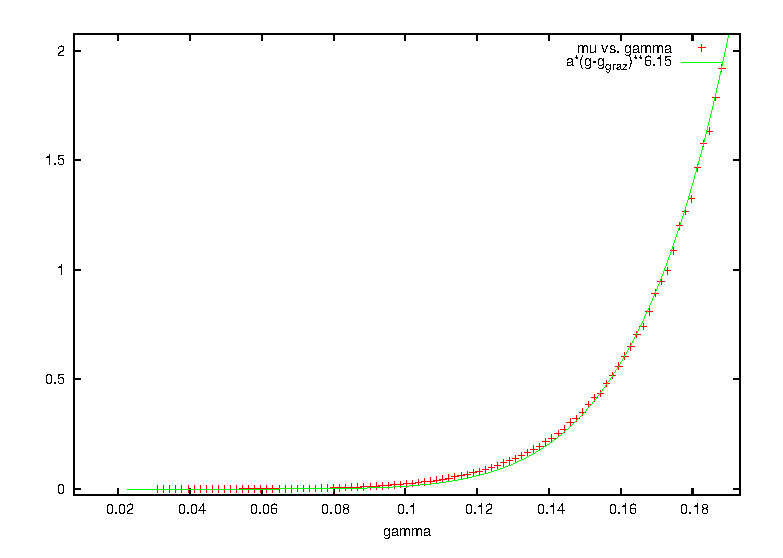
\includegraphics[width=0.8\columnwidth]{scang}
\end{center}
\end{figure}
\hyperlink{avgtvsg}{\beamergotobutton{back}}
\end{frame}

\begin{frame}
Celso Grebogi, Edward Ott, James A.   Yorke, Critical Exponent of 
Chaotic Transients in Nonlinear Dynamical Systems, Phys.   Rev.   Lett.   57, 
1284–1287 (1986):

\begin{problock}{Their results:}
\begin{itemize}
\item $\tau\sim(\alpha-\alpha_*)^{-\gamma}$, $\gamma$ the ``critical 
exponent'' depends on the system.  
\item Derives expression for $\gamma$ in terms of the eigenvalues of the fixed points at collision.  
\end{itemize}
\end{problock}

Drawing parallels between the behaviour of $\mu_{xv}$ and the previous result, we can surmise:
\[
\mu_{xv}\sim \frac{1}{\tau}
\]
\end{frame}



\begin{frame}{An approximate expression for the no-collision area $\mu_{xv}$}
So far, we have calculated $\mu_{xv}$ by means of a Monte Carlo integration: 
we chose $N$ initial points, evaluated the number $n$ of them that does 
not lead to collision and equated $\frac{n}{N}$ to $\mu_{xv}$.  \\

Now we'll try an analytical approach.  

\begin{align*}
\mu_{xv}&=\int_{A+B(x,v)e^{-\gamma t_c(x,v)/2}<\sigma}dxdv
\end{align*}


Now we recall \eqref{eq-tcol}
\begin{equation}
t_c= \left\{
\begin{matrix}
\frac{\pi-C}{\omega_g-\omega}\hspace{1em} \text{if }\omega_g>\omega\\
\frac{\pi+C}{\omega-\omega_g}\hspace{1em} \text{if }\omega_g<\omega
\end{matrix}
\right.  
\end{equation}
\end{frame}

\begin{frame}
Where $C=-tan^{-1}\frac{\frac{\gamma}{2\omega_g}x_0+\frac{v_0}{\omega_g}}{x_0}$.  

Since $C$ is a rapidly varying function of both $x$ and $v$ and has range 
$\left\{-\pi/2,\pi/2\right\}$, we can replace $C\approx 0$ without too much error.  \\

Therefore 
\begin{align*}
\mu_{xv}&\sim\int_{A+B(x,v)e^{-\gamma \pi/(2|\omega_g-\omega|)}<\sigma}dxdv\\
&=\int_{B(x,v)<(\sigma-A)e^{\gamma \pi/(2|\omega_g-\omega|)}}dxdv
\end{align*}

Now we recall that 
$B=\sqrt{x_0^2+\left(\frac{\gamma}{2\omega_g}x_0+\frac{v_0}{\omega_g}\right)^2}$
.  

So our integral is now of the form:
$\int_{x^2+(ax+by)^2<\chi^2}dxdv$
\end{frame}

\begin{frame}
\begin{align*}
&\int_{x^2+(ax+by)^2<\chi^2}dxdy\\
=&\int_{-\chi}^{\chi}dx\int_{x^2+(ax+by)^2<\chi^2} dy\\
=&\int_{-\chi}^{\chi} \frac{\sqrt{(2abx)^2-4b^2(x^2(1+a^2)-\chi^2)}}{b^2}   dx\\
=&\frac{1}{b^2}\int_{-\chi}^{\chi}2b\sqrt{\chi^2-x^2} dx\\
=&\frac{2}{b}\int_{-\chi}^{\chi}\sqrt{\chi^2-x^2} dx
\end{align*}

However, we have disregarded one very important restriction: $x<\sigma$, due to 
the hard wall.  \\

So, actually:
\begin{align*}
\mu_{xv}&=2\omega_g\int_{-\chi}^{max\{\chi,1\}} \sqrt{\chi^2-x^2}dx
\end{align*}

\end{frame}

\begin{frame}{Comparing the analytical result with Monte Carlo simulation}
\begin{figure}
\caption{$\mu_{vx}$ vs.  $F$}
\begin{center}
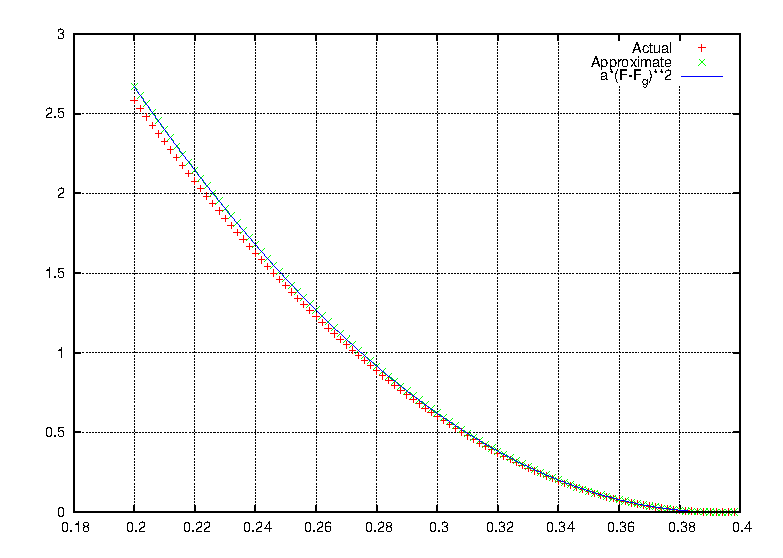
\includegraphics[width=0.75\columnwidth]{vxarea-actual-approx}
\end{center}
\end{figure}
\end{frame}


\begin{frame}[label=envelope-proof]{Attempt at justification of the envelope}
Recall that our calculation, both analytical and numerical, has started off 
with an assumption.   \hyperlink{envelope-guess}{\beamergotobutton{Envelope}}\\

Now we'll try to justify. \\
\begin{align*}
&\left|f(t)cos(\omega_1t)+g(t)cos(\omega_2t+C)\right|\\
\le&\left|(f(t)+g(t))(cos(\omega_1t)+cos(\omega_2t+C))\right|\\
=&2\left|\left\{f(t)+g(t)\right\}sin\left(\frac{(\omega_1-\omega_2)t+C}{2}\right)\right|\left|sin\left(\frac{(\omega_1+\omega_2)t+C}{2}\right)\right|
\end{align*}

Now since the last term is much more rapidly varying than the second term, we 
replace it with its average over a full cycle without incurring too much error:
\begin{align*}
=&2\left|\left\{f(t)+g(t)\right\}sin\left(\frac{(\omega_1-\omega_2)t+C}{2}\right)\right|\frac{2}{\pi}\int_0^{\pi/2}cos(t)dt\\
=&2\left|\left\{f(t)+g(t)\right\}sin\left(\frac{(\omega_1-\omega_2)t+C}{2}\right)\right|\frac{2}{\pi}
\end{align*}
\end{frame}

\begin{frame}{Nature of long lived transients}
\begin{figure}
\begin{center}
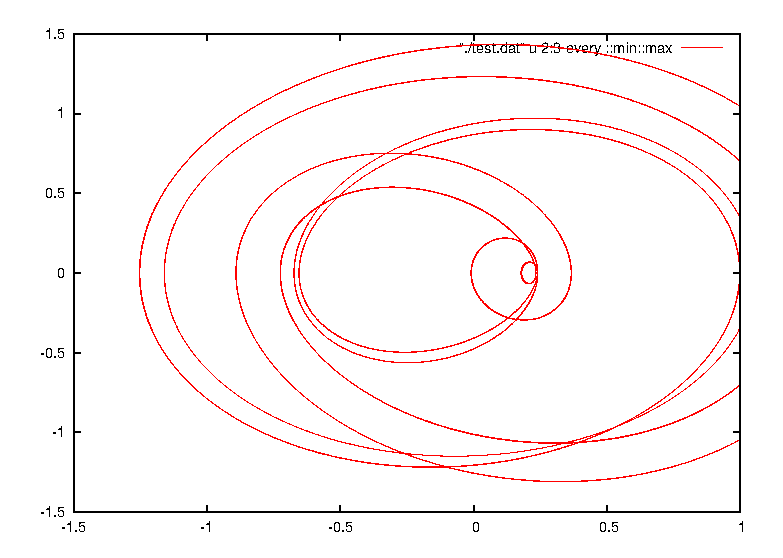
\includegraphics[width=0.8\columnwidth]{period_16_bfore_geazing_trajectory}
\end{center}
\end{figure}
\end{frame}

\begin{frame}{Nature of long lived transients}
\begin{figure}
\begin{center}
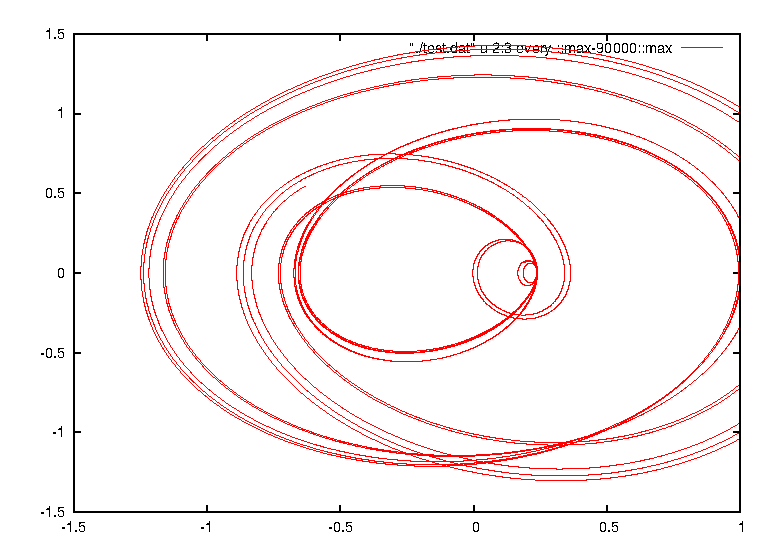
\includegraphics[width=0.8\columnwidth]{period_16_bfore_geazing_trajectory_mistaken}
\end{center}
\end{figure}
\end{frame}

\begin{frame}[label=envelope-am]
\em{$\omega >> \omega_g$}
\begin{eqnarray}
x(t)&=&-A\cos{\omega t}+e^{-\gamma t/2}B\cos{\left(\omega_g t+C\right)}\\
E(t)&=&A+e^{-\gamma t/2}B\cos{\left(\omega_g t+C\right)}
\end{eqnarray}

\begin{figure}
\begin{center}
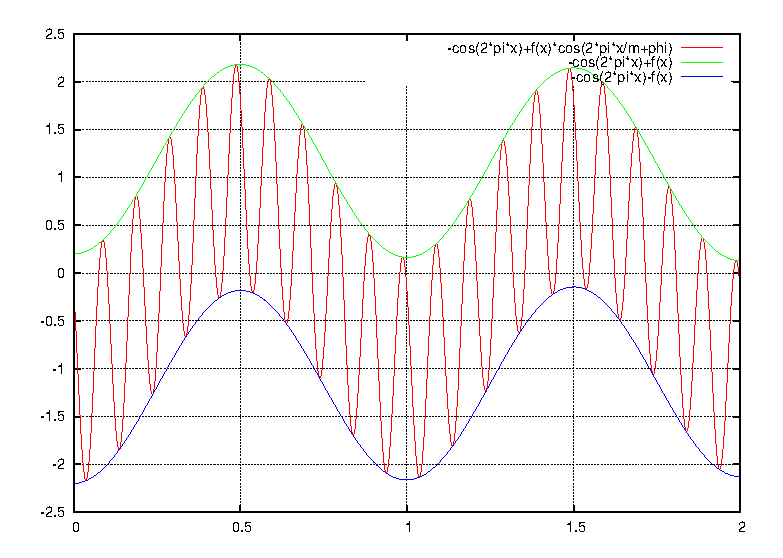
\includegraphics[width=0.8\columnwidth]{envelope-m-small}
\end{center}
\end{figure}
\end{frame}

\begin{frame}
\em{$\omega << \omega_g$}
\begin{eqnarray}
x(t)&=&-A\cos{\omega t}+e^{-\gamma t/2}B\cos{\left(\omega_g t+C\right)}\\
E(t)&=&-A\cos{\omega t}+e^{-\gamma t/2}B
\end{eqnarray}

\begin{figure}
\begin{center}
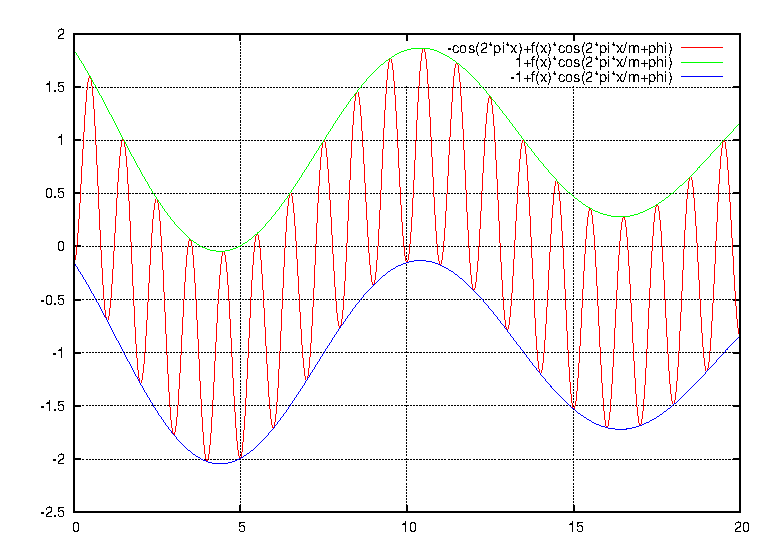
\includegraphics[width=0.8\columnwidth]{envelope-m-large}
\end{center}
\end{figure}
\end{frame}


\begin{frame}[label=avgtvsf]{Matching with lifetime data}
\begin{figure}
\caption{Transient lifetime vs.  $F$}
\begin{center}
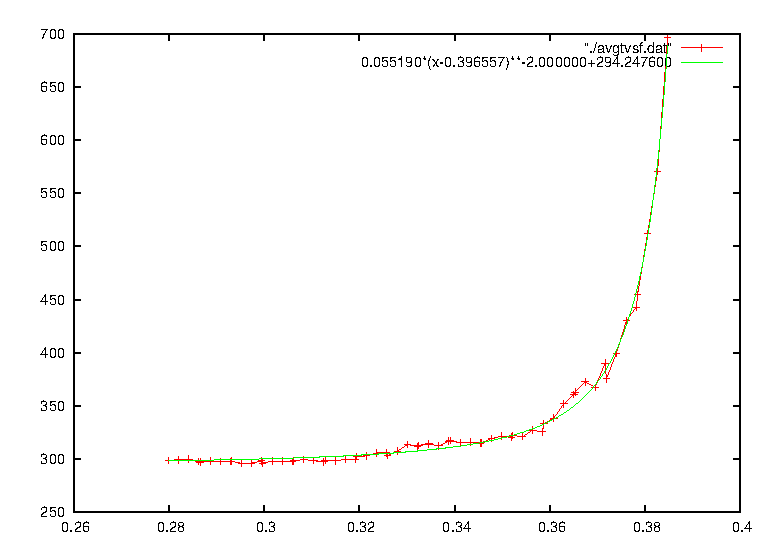
\includegraphics[width=0.8\columnwidth]{trans_life_vsf_matches}
\end{center}
\end{figure}
\hyperlink{muvsf}{\beamergotobutton{$\mu_{vx}$ vs. $F$}}
\end{frame}

\begin{frame}[label=avgtvsg]
\begin{figure}
\caption{Transient lifetime vs.  $\gamma$}
\begin{center}
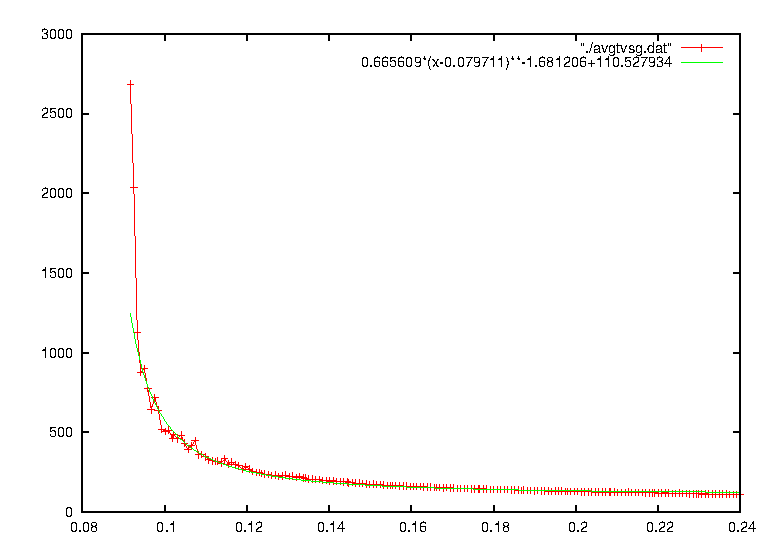
\includegraphics[width=0.8\columnwidth]{trans_life_vsg_matches_somewhat}
\end{center}
\end{figure}
\hyperlink{muvsg}{\beamergotobutton{$\mu_{vx}$ vs. $\gamma$}}
\end{frame}

\begin{frame}
\begin{figure}
\caption{Transient lifetime vs.  $r$}
\begin{center}
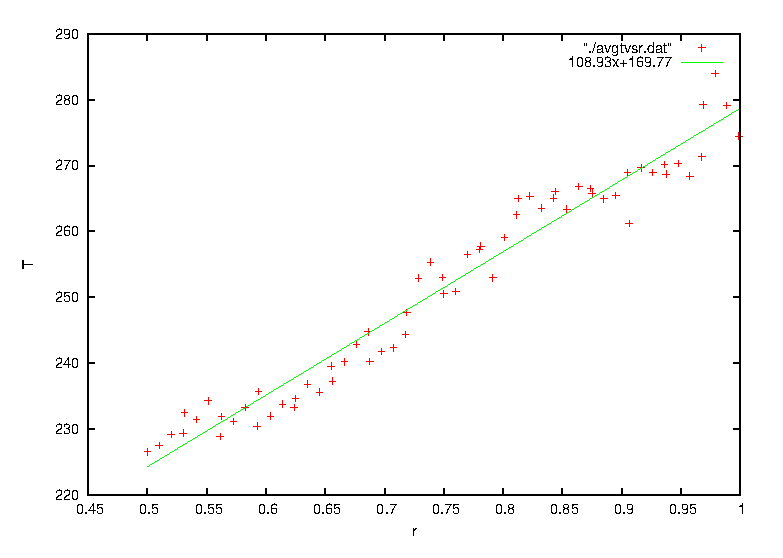
\includegraphics[width=0.8\columnwidth]{trans_life_vsr}
\end{center}
\end{figure}
\end{frame}


\begin{frame}<article>{TODO}
\begin{enumerate}
\item Try to squeeze the parallelogram shaped bounding box of $\mu_{xv}$.  
\item Create a colourmap of $\mathbb{V\times X}$ space depicting the number of 
cycles needed to reach stable period-1 orbit.  
\item Instead of Monte Carlo integration, try a spreading-out approach.  
\item As per Grebogi, Yorke et al, try to find out the ``critical exponent''
\item The other extreme: $\omega_0>>\omega$ or $\omega_0<<\omega$ 
\item Prove that the peak of $e^{-\gamma t/2}cos(\omega t)$ doesn't differ 
markedly from that of $cos(\omega t)$
\end{enumerate}
\end{frame}



\end{document}
